\section{Getting Started with \index{BPi}{BPi}}

Inspired and encouraged by success of Raspberry Pi, Banana Pi is another attemtp to create a small yet powerful computer board. TBC.

\begin{figure}[H]
\caption{SoC Computer board}
\label{fig:SoC computers}
\begin{center}
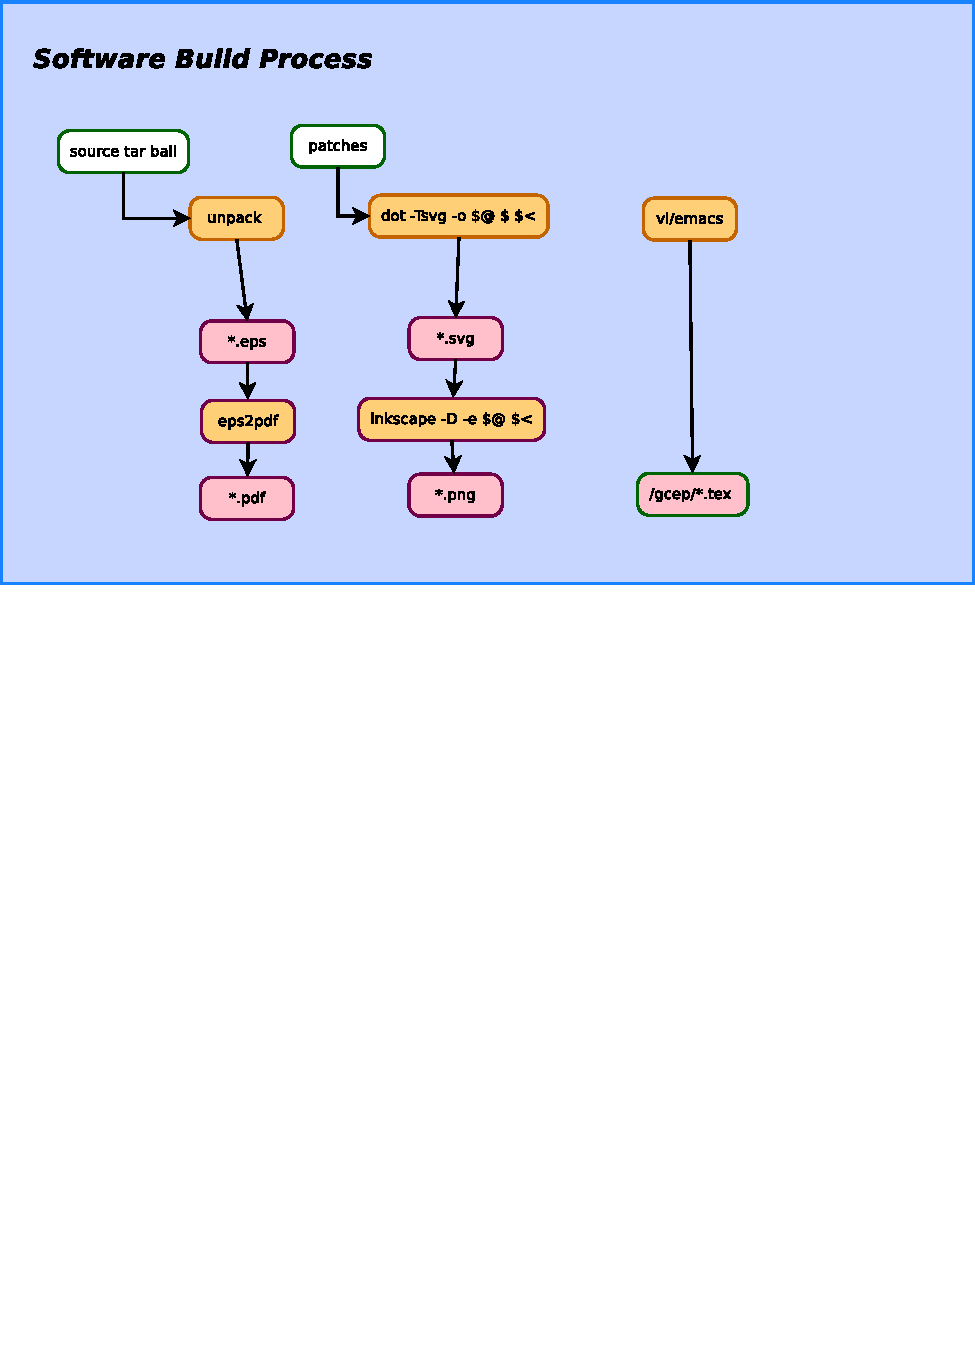
\includegraphics[scale=0.65]{dia/sbutils.pdf}
\end{center}
\end{figure}

\subsection{Using Unix dd command to flash Lbunutu image}

\begin{enumerate}
\item As shown in following log, Lubuntu 14.04 version 3.0 got written into /dev/sdc.
\begin{Verbatim} [frame=lines,framesep=5mm,label={[Start of code] End of code}]
root@bpi01:/pub# dd bs=4M if=/pub/Lubuntu_1404_For_BananaPi_v3_0.img  of=/dev/sdc
120+0 records in
120+0 records out
503316480 bytes (503 MB) copied, 45.0463 s, 11.2 MB/s
875+0 records in
875+0 records out
3670016000 bytes (3.7 GB) copied, 373.487 s, 9.8 MB/s
root@bpi01:/pub# 
\end{Verbatim}

\item Use sb tool to test build hello-2.7
  \begin{lstlisting}
TJYANG-MBA:~ tjyang\$ sb -

TJYANG-MBA:~ tjyang\$ tail -1 ~/.bashrc

  \end{lstlisting}

\item sbutils -version
  \begin{lstlisting}
tjyang@tj1210:~/gcep$ which sbutils
tjyang@tj1210:~/gcep$ 
  \end{lstlisting}
\end{enumerate}

